\section{Historias de usuario}
\setlength{\parindent}{2em}
Las historias de usuario, son pequeñas descripciones de los requerimientos de un cliente. Su utilización es común cuando se aplica marcos de entornos ágiles como SCRUM. 

Al redactar las historias de usuario se debe tener en cuenta describir el Rol, la funcionalidad y el resultado esperado en una frase corta. Debe venir acompañada de los criterios de aceptación.

Es deseable que las historias de usuario sean escritas por el usuario, en una frase corta. Debe describir el rol desempeñado por el usuario de forma explícita e indicar el beneficio para el área de negocio que representa esta funcionalidad. 

\subsection{Listado de historias de usuario}

\begin{shaded}
	\underline{\textbf{Historia 1:}}
	\begin{flushleft}	
		\textbf{Como:} Cliente.\\
		\textbf{Quiero:} Analizar el know how de la empresa.\\
		\textbf{Para:} Estudiar la mejor forma de adaptar los requisitos a la forma de trabajar de la empresa.\\ 
	\end{flushleft}			
\end{shaded}

\begin{shaded}
	\underline{\textbf{Historia 2:}}
	\begin{flushleft}	
		\textbf{Como:} Cliente.\\
		\textbf{Quiero:} Disponer de un listado de clientes offline.\\
		\textbf{Para:} Tener a disposición los clientes sin necesidad de estar conectado.\\ 
	\end{flushleft}			
\end{shaded}

\begin{shaded}
	\underline{\textbf{Historia 3:}}
	\begin{flushleft}	
		\textbf{Como:} Cliente.\\
		\textbf{Quiero:} Disponer de un listado de productos offline.\\
		\textbf{Para:} Tener a disposición los productos sin necesidad de estar conectado.\\ 
	\end{flushleft}			
\end{shaded}

\clearpage

\begin{shaded}
	\underline{\textbf{Historia 4:}}
	\begin{flushleft}	
		\textbf{Como:} Cliente.\\
		\textbf{Quiero:} Disponer de un listado de pedidos por cliente offline.\\
		\textbf{Para:} Tener a disposición los pedidos realizados por un cliente sin necesidad de estar conectado.\\ 
	\end{flushleft}			
\end{shaded}

\begin{shaded}
	\underline{\textbf{Historia 5:}}
	\begin{flushleft}	
		\textbf{Como:} Cliente.\\
		\textbf{Quiero:} Poder crear pedidos por cliente.\\
		\textbf{Para:} Gestionar en la aplicación los pedidos y tenerlos almacenados.\\ 
	\end{flushleft}			
\end{shaded}

\begin{shaded}
	\underline{\textbf{Historia 6:}}
	\begin{flushleft}	
		\textbf{Como:} Cliente.\\
		\textbf{Quiero:}  Poder editar los pedidos no enviados.\\
		\textbf{Para:} Realizar correcciones antes de enviar los pedidos.\\ 
	\end{flushleft}			
\end{shaded}

\begin{shaded}
	\underline{\textbf{Historia 7:}}
	\begin{flushleft}	
		\textbf{Como:} Cliente.\\
		\textbf{Quiero:} Tener listados de productos por pedido.\\
		\textbf{Para:} Visualizar los productos y gestionar filtros.\\ 
	\end{flushleft}			
\end{shaded}

\begin{shaded}
	\underline{\textbf{Historia 8:}}
	\begin{flushleft}	
		\textbf{Como:} Cliente.\\
		\textbf{Quiero:} Poder enviar los pedidos realizados a la central.\\
		\textbf{Para:} Disponer de una interface que comunique con la la aplicación de gestión.\\ 
	\end{flushleft}			
\end{shaded}

 \clearpage
 
\begin{shaded}
	\underline{\textbf{Historia 9:}}
	\begin{flushleft}	
		\textbf{Como:} Cliente.\\
		\textbf{Quiero:} Completa abstracción de la app vs aplicación de gestión.\\
		\textbf{Para:} No modificar en la medida de lo posible el producto usado hasta ahora, y mantener la forma de trabajar.\\ 
	\end{flushleft}			
\end{shaded} 


\begin{shaded}
	\underline{\textbf{Historia 10:}}
	\begin{flushleft}	
		\textbf{Como:} Cliente.\\
		\textbf{Quiero:} probar la funcionalidad.\\
		\textbf{Para:} tener un tiempo de pruebas para verificar la funcionalidad de la app.\\ 
	\end{flushleft}			
\end{shaded} 

\section{Product Backlog}

Se estima que la realización del proyecto tendrá una estimación de 5 Iteraciones (2 semanas por iteración) para la fase de desarrollo y 1 Iteración adicional para testeo y pruebas finales con el cliente. Se ha concretado con el cliente unas funcionalidades a través de las historias de usuario. Dejando para una fase posterior, fuera de esta planificación y por ende fuera de este proyecto, Modificaciones adicionales o sugerencias por parte del cliente. 

La jornada diaria tendrá un valor de 1 punto correspondiendo este a una jornada laboral de 8h/dia. Así pues una iteración dispondrá de 10 puntos, que equivalen a los 10 dias laborables incluidos en las dos semanas descritas.

\begin{figure}[H]
	\centering
	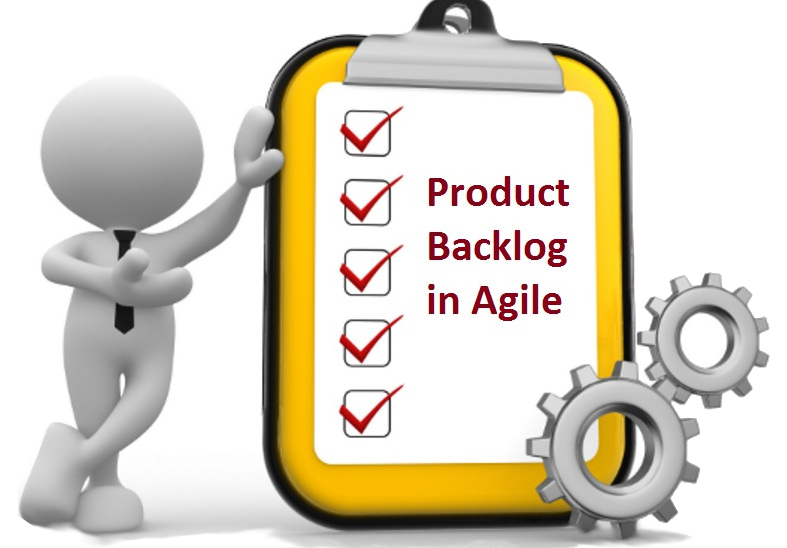
\includegraphics[width=0.55\linewidth]{figuras/spring}
	\label{fig:spring}
\end{figure}

A continuación en la Tabla 4.1 se detalla el Product Backlog inicial, con las historias  de usuario a implementar priorizadas según las necesidades detectadas por el equipo de desarrollo y el Director del proyecto. 

\begin{table}[H]
	\centering
	\caption{Product backlog}
	\label{Product backlog}
	\renewcommand{\arraystretch}{2}
	\begin{tabular}{cccc}
		\multicolumn{4}{c}{\cellcolor{tittletable}{\color{white} \textbf{Product Backlog}}} \\
		\rowcolor{HeaderCol} 
		{\color{white} \textbf{ID}} & {\color{white}  \textbf{Nombre historia}} & {\color{white} \textbf{Estimación}} & {\color{white} \textbf{Prioridad}} \\ 
		\hline
		
		\multicolumn{1}{|c|}{1} & \multicolumn{1}{l|}{Analizar el know how de la empresa} & \multicolumn{1}{c|}{10} & \multicolumn{1}{c|}{Media} \\ \hline
		
		\multicolumn{1}{|c|}{2} & \multicolumn{1}{l|}{Disponer de un listado de clientes offline} & \multicolumn{1}{c|}{5} & \multicolumn{1}{c|}{Media} \\ \hline
	
		\multicolumn{1}{|c|}{3} & \multicolumn{1}{l|}{Disponer de un listado de pedidos por cliente offline} & \multicolumn{1}{c|}{5} & \multicolumn{1}{c|}{Media} \\ \hline
			
		\multicolumn{1}{|c|}{4} & \multicolumn{1}{l|}{Disponer de un listado de productos offline} & \multicolumn{1}{c|}{5} & \multicolumn{1}{c|}{Media} \\ \hline
			
		\multicolumn{1}{|c|}{5} & \multicolumn{1}{l|}{Poder crear pedidos por cliente} & \multicolumn{1}{c|}{8} & \multicolumn{1}{c|}{Alta} \\ \hline
				
		\multicolumn{1}{|c|}{6} & \multicolumn{1}{l|}{Poder editar los pedidos no enviados.} & \multicolumn{1}{c|}{8} & \multicolumn{1}{c|}{Alta} \\ \hline
					
		\multicolumn{1}{|c|}{7} & \multicolumn{1}{l|}{Tener listados de productos por pedido} & \multicolumn{1}{c|}{5} & \multicolumn{1}{c|}{Alta} \\ \hline
						
		\multicolumn{1}{|c|}{8} & \multicolumn{1}{l|}{Poder enviar los pedidos realizados a la central} & \multicolumn{1}{c|}{5} & \multicolumn{1}{c|}{Alta} \\ \hline
		
		\multicolumn{1}{|c|}{9} & \multicolumn{1}{l|}{Completa abstracción de la app vs aplicación de gestión} & \multicolumn{1}{c|}{2} & \multicolumn{1}{c|}{Baja} \\ \hline
		
		\multicolumn{1}{|c|}{10} & \multicolumn{1}{l|}{Probar la funcionalidad} & \multicolumn{1}{c|}{2} & \multicolumn{1}{c|}{Alta} \\ \hline
	\end{tabular}
\end{table}

\clearpage

Más adelante en la Tabla 4.2 se muestra la planificación de las iteraciones con sus respectivas historias y objetivos a cumplir en cada ciclo. 

\begin{table}[H]
	\centering
	\caption{Iteraciones}
	\label{Iteraciones}
	\renewcommand{\arraystretch}{2}
	
	\begin{tabular}{cccccc}
		\multicolumn{6}{c}{\cellcolor{tittletable}{\color{white} \textbf{Iteraciones}}} \\
		\rowcolor{HeaderCol} 
		{\color{white} \textbf{Ite.}} & {\color{white}  \textbf{Inicio}} & {\color{white} \textbf{Fin}} & {\color{white} \textbf{Historias}}  & {\color{white} \textbf{Puntos}} & {\color{white} \textbf{Objetivos}}\\ 
		\hline
		
		\multicolumn{1}{|c|}{1} & \multicolumn{1}{l|}{01/01/2018} 
		& \multicolumn{1}{c|}{12/01/2018} & \multicolumn{1}{c|}{1} 
		& \multicolumn{1}{c|}{10}  & \multicolumn{1}{p{6cm}|}{	
			Analizar como recuperar los datos a procesar.
			Analizar como se insertan los pedidos en la aplicación de gestión existente.
			Ver y plantear la Querys necesarias para operar la DB.
			Iniciar la generación del servicio web que va a comunicar con la BD.
		} \\ \hline
		\multicolumn{1}{|c|}{2} & \multicolumn{1}{l|}{15/01/2018} 
		& \multicolumn{1}{c|}{26/01/2018} & \multicolumn{1}{c|}{2} 
		& \multicolumn{1}{c|}{10}  & \multicolumn{1}{p{5.0cm}|}{
			Desarrollar conjunto para realizar sincronización de datos.	
			Aplicar métodos de consulta al servicio web.
		} \\ \hline
		
		\multicolumn{1}{|c|}{3} & \multicolumn{1}{l|}{29/01/2018} 
		& \multicolumn{1}{c|}{09/02/2018} & \multicolumn{1}{c|}{1.8} 
		& \multicolumn{1}{c|}{10}  & \multicolumn{1}{p{5.0cm}|}{
			Desarrollar conjunto para realizar pedidos.	
			Aplicar métodos de consulta al servicio web.
			Aplicar métodos de inserción al servicio web.
		} \\ \hline
		
		\multicolumn{1}{|c|}{4} & \multicolumn{1}{l|}{12/02/2018} 
		& \multicolumn{1}{c|}{23/02/2018} & \multicolumn{1}{c|}{1.7} 
		& \multicolumn{1}{c|}{10}  & \multicolumn{1}{p{5.0cm}|}{
			Desarrollar conjunto para editar pedidos no enviados.
			Desarrollar conjunto para ver pedidos no previos. 
			Aplicar métodos de consulta al servicio web.
		} \\ \hline
		
		\multicolumn{1}{|c|}{5} & \multicolumn{1}{l|}{26/01/2018} 
		& \multicolumn{1}{c|}{09/03/2018} & \multicolumn{1}{c|}{2.5} 
		& \multicolumn{1}{c|}{10}  & \multicolumn{1}{p{5.0cm}|}{
			Terminar la generación del servicio web. 		
		} \\ \hline
		
		\multicolumn{1}{|c|}{6} & \multicolumn{1}{l|}{12/03/2018} 
		& \multicolumn{1}{c|}{23/03/2018} & \multicolumn{1}{c|}{1} 
		& \multicolumn{1}{c|}{10}  & \multicolumn{1}{p{5.0cm}|}{
			Pruebas de funcionamiento.
		} \\ \hline

	\end{tabular}

\end{table}

\section{Estimación de costes del proyecto}

Teniendo en cuenta los datos anteriores podemos estimar los siguiente recursos de trabajo:
	\begin{itemize}
		\item \textbf{Trabajo total estimado:} 480 horas.
		\item \textbf{Coste pactado:}  6.999 €.
		\item \textbf{Coste hora:} 14,58 € /h.
	\end{itemize}

\subsection{Cálculo de costes del proyecto}

\subsubsection{Recursos de trabajo}

Analista/Programador informático: $ 28.000 \euro / 14p  / 20d  / 8h = 12.5 \euro/h $ 

\subsubsection{Recursos materiales}

Los recursos materiales se consideran cada uno de ellos con un coste por uso de 1,50\euro en concepto de luz y otros gastos que se cobran independientemente del tiempo de uso: $60d \times 1.50\euro= 90\euro$ 

\begin{table}[H]
	\centering
	\caption{Software}
	\label{Software}
	\renewcommand{\arraystretch}{2}
	
	\begin{tabular}{ccc}
		\multicolumn{3}{c}{\cellcolor{tittletable}{\color{white} \textbf{Software}}} \\
		\rowcolor{HeaderCol} 
		{\color{white} \textbf{Concepto}} & {\color{white} \textbf{Coste}} & {\color{white} \textbf{Licencias}}\\ 
		\hline
		
		\multicolumn{1}{|p{6cm}|}{MS Windows 10} & \multicolumn{1}{r|}{149,00\euro} 
		& \multicolumn{1}{c|}{1}\\ \hline
		
		\multicolumn{1}{|p{6cm}|}{Text Studio 2.12} & \multicolumn{1}{r|}{0,00\euro} 
		& \multicolumn{1}{c|}{1}\\ \hline
		
		\multicolumn{1}{|p{6cm}|}{Gimp 2.8} & \multicolumn{1}{r|}{0,00\euro} 
		& \multicolumn{1}{c|}{1}\\ \hline
		
		\multicolumn{1}{|p{6cm}|}{Eclipse oxygen} & \multicolumn{1}{r|}{0,00\euro} 
		& \multicolumn{1}{c|}{1}\\ \hline
		
		\multicolumn{1}{|p{6cm}|}{Android Studio 3.1} & \multicolumn{1}{r|}{0,00\euro} 
		& \multicolumn{1}{c|}{1}\\ \hline
		
	\end{tabular}
	
\end{table}

\subsubsection{Costes totales}
En la siguiente lista se detallan los costes del proyecto. Aunque a priori parezcan que son deficitarios con una desviación de 853\euro en perdidas, hay que tener en cuenta que la figura del analista programador y el gestor del proyecto es la misma y las perdidas son absorbidas por su remuneración.  

\begin{figure}[H]
	\centering
	\begin{tabular}{lr}
		\textbf{Concepto} & \textbf{Coste} \\ \hline \\
		Trabajo & 6.000,00\euro \\
		Materiales	& 240,00\euro \\
		Total & 6.240,00\euro \\
		Gastos(4) & 249,60\euro \\
		Subtotal & 6.489,60\euro \\
		IVA(18)	& 1.362,82\euro \\
		Total & 7852,42\euro \\ \hline
		
	\end{tabular} 
\end{figure}

\section{Seguimiento del Proyecto}

\subsection{1º Iteración}
Durante la primera iteración, se proyecta realizar el análisis correspondiente de la aplicación cliente y sus posibles implicaciones posteriores. La aplicación cliente se encuentra en un servidor centralizado con una base de datos relacional PostgreSQL.
En principio se tiene bastante claro que datos se tienen que recoger y con que formato se insertan los pedidos en la misma. Se desarrollan consultas \textit{(query)} SQL\textsl{} previas para su uso posterior.
\subsubsection{Comentarios y conclusiones }
No hay desviaciones aparentes y se encuentra en plazo.

\subsection{2º Iteración}
En la segunda iteración se trabaja en la gestión de los listados y el esqueleto de las dos aplicaciones, se ha definido la comunicación y la manera de operar de las mismas. 
\subsubsection{Comentarios y conclusiones }
Aparece una ligera desviación que se presupone será incremental en las subsiguientes iteraciones. Hay una pequeña linea difusa entre los diferentes listados que origina la 
creación de código que a priori esta planificado para iteraciones posteriores.
\subsection{3º Iteración}
En la tercera iteración estaba planificado el desarrollo primario de la gestión de pedidos. Durante la creación de las pantallas básicas no se había tenido en cuenta el tiempo de creación de los iconos e imágenes del sistema.
\subsubsection{Comentarios y conclusiones }
El diseño de la apariencia de la aplicación  Android no se había tenido en cuenta, así pues se dedica una parte importante de la iteración a realizar todos los diseños que vamos a necesitar, tanto para esta iteración como para las posteriores. Se espera absorber este tiempo en iteraciones posteriores.
\subsection{4º Iteración}
Se procede al desarrollo de código fuente para gestionar los pedidos al completo
\subsubsection{Comentarios y conclusiones }
La elección de tecnologías de desarrollo ágiles como el proyecto Lombok, o AndroidAnnotations, que simplifican la generación de código, permiten absorber las desviaciones temporales acarreadas por las iteraciones posteriores.
\subsection{5º Iteración}
Se finalizan algunas funcionalidades pendientes y se termina el servicio web para gestionar los datos a enviar/recibir.
\subsubsection{Comentarios y conclusiones }
Como estamos por debajo de la estimación se aprovecha para realizar una instalación previa y algunas pruebas.   
\subsection{6º Iteración}
Durante esta Iteración, se realizan pruebas unitarias, de integración y funcionales con el cliente, identificando ligeros fallos que se corrigen durante la duración de esta iteración.  

\subsection{Final de iteraciones}
Una vez extrapolados los datos obtenidos por el tablón de seguimiento, obtenemos unas gráficas que muestran las desviaciones generadas por los diferentes escollos que se han generado durante el desarrollo de la aplicación 

En la siguiente gráfica podemos ver la desviación por iteración:\\
	
\begin{figure}[H]
	\centering
	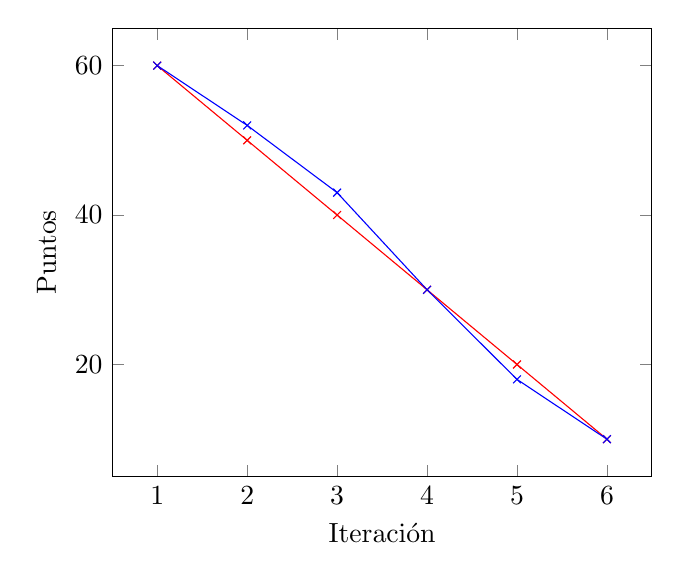
\begin{tikzpicture} 
		\begin{axis}[ xlabel=Iteración, ylabel=Puntos] 

			\addplot[color=red,mark=x] coordinates { (1,60) (2,50) (3,40) (4,30) (5,20) (6,10)};

			\addplot[color=blue,mark=x] coordinates { (1,60) (2,52) (3,43) (4,30) (5,18) (6,10)};
	
		\end{axis} 
	\end{tikzpicture}
	\captionof{figure}{Product Burn-Down}
	\label{tikz-1}
\end{figure}

\clearpage

En la siguiente gráfica podemos ver la desviación por Iteraciones/día:\\

\begin{figure}[H]
	\centering
	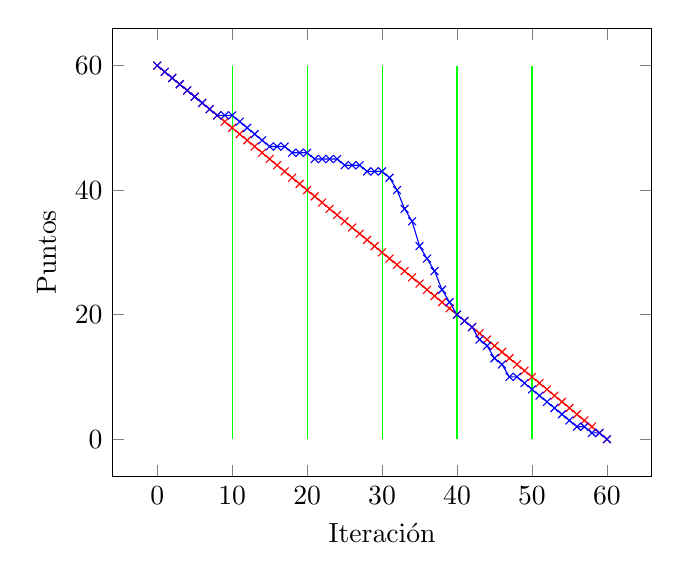
\begin{tikzpicture} 
		\begin{axis}[ xlabel=Iteración, ylabel=Puntos] 

			\addplot[color=red,mark=x] coordinates { (0,60) (1,59) (2,58) (3,57) (4,56) (5,55)
				(6,54) (7,53) (8,52) (9,51) (10,50) (11,49) (12,48) (13,47) (14,46) (15,45) (16,44) (17,43) (18,42) (19,41) (20,40) (21,39) (22,38) (23,37) (24,36) (25,35)
				(26,34) (27,33) (28,32) (29,31) (30,30) (31,29) (32,28) (33,27) (34,26) (35,25) (36,24) (37,23) (38,22) (39,21) (40,20) (41,19) (42,18) (43,17) (44,16) (45,15)
				(46,14) (47,13) (48,12) (49,11) (50,10) (51,9) (52,8) (53,7) (54,6) (55,5)
				(56,4) (57,3) (58,2) (59,1) (60,0)};
			
			\addplot[color=blue,mark=x] coordinates { (0,60) (1,59) (2,58) (3,57) (4,56) (5,55)
				(6,54) (7,53) (8,52) (9,52) (10,52) (11,51) (12,50) (13,49) (14,48) (15,47) (16,47) (17,47) (18,46) (19,46) (20,46) (21,45) (22,45) (23,45) (24,45) (25,44)
				(26,44) (27,44) (28,43) (29,43) (30,43) (31,42) (32,40) (33,37) (34,35) (35,31) (36,29) (37,27) (38,24) (39,22) (40,20) (41,19) (42,18) (43,16) (44,15) (45,13)
				(46,12) (47,10) (48,10) (49,9) (50,8) (51,7) (52,6) (53,5) (54,4) (55,3)
				(56,2) (57,2) (58,1) (59,1) (60,0)};
			
			\addplot[color=green] coordinates { (10,0) (10,60)};
			\addplot[color=green] coordinates { (20,0) (20,60)};
			\addplot[color=green] coordinates { (30,0) (30,60)};
			\addplot[color=green] coordinates { (40,0) (40,60)};
			\addplot[color=green] coordinates { (50,0) (50,60)};
		\end{axis} 
	\end{tikzpicture}
	\captionof{figure}{Sprints BurnDown}
	\label{tikz-2}
\end{figure}

